% Gatekeeper -- EASE 2027 research paper (anonymous, ACM sigconf; 10 pages including appendices,
% up to 2 pages of references). Numbers in the text: paper/numbers.tex (scripts/make_numbers.py);
% bibliography: paper/refs.bib (scripts/make_bib.py). None is edited by hand.
\documentclass[sigconf,review,anonymous]{acmart}
\acmConference[EASE 2027]{The 31st International Conference on Evaluation and Assessment in Software Engineering}{15--18 June, 2027}{Hanoi, Vietnam}
\settopmatter{printacmref=false}
\setcopyright{none}
\renewcommand\footnotetextcopyrightpermission[1]{}
\usepackage{booktabs}
\usepackage{tikz}
\usetikzlibrary{arrows.meta,positioning,calc}
\usepackage{pgfplots}
\pgfplotsset{compat=1.18}

\newtheorem{assumption}{Assumption}
\newcommand{\STR}{\mathrm{STR}}
% The one place where the agent's model is named in the text (exact version: replication package).
\newcommand{\agentmodel}{Gemini~3.1 Flash-Lite}
\newcommand{\promodel}{Gemini~3.1 Pro (preview)}
\newcommand{\flashmodel}{Gemini~3.8 Flash}
% Every number in the text is a macro generated from results/ by scripts/make_numbers.py.
% Generated by scripts/make_numbers.py from results files. Do not edit by hand.
\newcommand{\njinjaNone}{15}
\newcommand{\njinjaSkill}{53}
\newcommand{\njinjaGain}{0.38}
\newcommand{\njinjaGainLo}{0.26}
\newcommand{\njinjaGainHi}{0.49}
\newcommand{\njinjaAdmit}{29}
\newcommand{\njinjaLNone}{37}
\newcommand{\njinjaLSkill}{79}
\newcommand{\njinjaLFNone}{14}
\newcommand{\njinjaLFSkill}{35}
\newcommand{\njinjaLFGain}{0.21}
\newcommand{\njinjaLFGainLo}{0.13}
\newcommand{\njinjaLFGainHi}{0.29}
\newcommand{\njinjaLFAdmit}{50}
\newcommand{\njinjaLFp}{\ensuremath{4.8\times10^{-7}}}
\newcommand{\nleak}{0.17}
\newcommand{\nleakLo}{0.06}
\newcommand{\nleakHi}{0.28}
\newcommand{\nleakShare}{0.45}
\newcommand{\njinjaNoPSn}{15}
\newcommand{\njinjaNoPSLF}{0}
\newcommand{\njinjaNoPSTasks}{34}
\newcommand{\njinjaWithPSGain}{24}
\newcommand{\njinjaWithPSLFGain}{21}
\newcommand{\nbleveNone}{13}
\newcommand{\nbleveSkill}{43}
\newcommand{\nbleveGain}{0.30}
\newcommand{\nbleveGainLo}{0.19}
\newcommand{\nbleveGainHi}{0.40}
\newcommand{\nbleveAdmit}{34}
\newcommand{\nbleveLNone}{30}
\newcommand{\nbleveLSkill}{73}
\newcommand{\nbleveNoPS}{11}
\newcommand{\nbleveNoPSNone}{0}
\newcommand{\nfzeroLNoop}{206}
\newcommand{\nfzeroSNoop}{0}
\newcommand{\nfzeroN}{216}
\newcommand{\nfzeroRepos}{5}
\newcommand{\nnoopOurs}{0}
\newcommand{\nnoopOursN}{40}
\newcommand{\ngoldOursOk}{33}
\newcommand{\ngoldOursN}{35}
\newcommand{\netwoGain}{0.02}
\newcommand{\ntfourGain}{0.60}
\newcommand{\nsskbRho}{0.07}
\newcommand{\nsskbOpp}{0.19}
\newcommand{\npluginOnce}{0.46}
\newcommand{\npluginMonitored}{0.80}
\newcommand{\ngepaNoop}{0.14}
\newcommand{\ngkAdmitAA}{0.0032}
\newcommand{\nattrTasks}{109}
\newcommand{\nattrSkill}{13}
\newcommand{\nattrPlacebo}{14}
\newcommand{\nattrR}{1.08}
\newcommand{\nattrRLo}{0.68}
\newcommand{\nattrRHi}{1.75}
\newcommand{\nshamLite}{0.51}
\newcommand{\nshamFlash}{0}
\newcommand{\nshamPro}{0.09}
\newcommand{\nnoiseWithin}{7}
\newcommand{\nnoiseClaims}{13}
\newcommand{\nnoiseTasks}{257}
\newcommand{\nbxOnce}{0.03}
\newcommand{\nbxMonitored}{0.11}
\newcommand{\nlibDrift}{0.0030}
\newcommand{\neSR}{1.00}
\newcommand{\ngkRetire}{0.0018}
\newcommand{\netwoS}{0.02}
\newcommand{\netwoF}{0.01}
\newcommand{\netwoB}{0.02}
\newcommand{\ntfourS}{0.55}
\newcommand{\ntfourF}{0.65}
\newcommand{\neoneFlips}{3}
\newcommand{\neoneSides}{1540}
\newcommand{\netwoFlips}{0}
\newcommand{\netwoSides}{30}
\newcommand{\nrescoredPatches}{1200}
\newcommand{\nproPairs}{8}
\newcommand{\nproSame}{8}
\newcommand{\nproNoneMedian}{0.93}
\newcommand{\nsskbSame}{0.25}
\newcommand{\nsskbSamePct}{25}
\newcommand{\nsskbConfigs}{4}
\newcommand{\nsskbSkills}{98}
\newcommand{\ndriftMatch}{74}
\newcommand{\ndriftTasks}{109}
\newcommand{\nblockedGold}{5}
\newcommand{\nsskbThr}{6}
\newcommand{\nplcS}{24}
\newcommand{\nconGain}{0.29}
\newcommand{\nconGainLo}{0.18}
\newcommand{\nconGainHi}{0.40}
\newcommand{\nconP}{\ensuremath{2.4\times10^{-6}}}
\newcommand{\nconAdmit}{50}
\newcommand{\nconWithPSSkill}{38}
\newcommand{\nconWithPSPlc}{24}
\newcommand{\nconWithPSp}{0.0047}
\newcommand{\nplcNoPS}{0}
\newcommand{\nlenGain}{0.09}
\newcommand{\nlenGainLo}{0}
\newcommand{\nlenGainHi}{0.18}
\newcommand{\nlenP}{0.09}
\newcommand{\ntrTasks}{34}
\newcommand{\ntrGitCmd}{34}
\newcommand{\ntrBugPatch}{34}
\newcommand{\ntrSolved}{15}
\newcommand{\ntrSame}{30}
\newcommand{\ntrN}{34}
\newcommand{\njinjaNoPSNoneBase}{1}
\newcommand{\ngoNoneTraced}{100}
\newcommand{\ngoNoneCmd}{91}
\newcommand{\ngoNoneErr}{68}
\newcommand{\ngoSkillTraced}{98}
\newcommand{\ngoSkillCmd}{28}
\newcommand{\ngoSkillErr}{3}
\newcommand{\ngoHitNone}{9}
\newcommand{\ngoHitSkill}{14}
\newcommand{\ngoRestN}{32}
\newcommand{\ngoRestNone}{5}
\newcommand{\ngoRestSkill}{17}
\newcommand{\nbleveCrash}{2}
\newcommand{\nbleveSiN}{98}
\newcommand{\nbleveSiB}{19}
\newcommand{\nbleveSiC}{2}
\newcommand{\nbleveSiGain}{0.17}
\newcommand{\nbleveSiLeak}{0.12}
\newcommand{\nbleveLFNone}{14}
\newcommand{\nbleveLFSkill}{31}
\newcommand{\nbleveLFGain}{0.17}
\newcommand{\nbleveLFGainLo}{0.09}
\newcommand{\nbleveLFGainHi}{0.25}
\newcommand{\nbleveLFp}{\ensuremath{1.1\times10^{-4}}}
\newcommand{\nbleveLFAdmit}{61}
\newcommand{\nbleveLFLNone}{31}
\newcommand{\nbleveLFLSkill}{59}
\newcommand{\nbleveNoPSLF}{0}
\newcommand{\nbleveNoPSN}{42}
\newcommand{\nbleveLeak}{0.13}
\newcommand{\nbleveLeakLo}{0.03}
\newcommand{\nbleveLeakHi}{0.23}
\newcommand{\nbleveLeakSharePct}{43}
\newcommand{\nbleveTrTasks}{100}
\newcommand{\nbleveTrGitCmd}{31}
\newcommand{\nbleveTrBugPatch}{0}
\newcommand{\npygN}{100}
\newcommand{\npygSkill}{6}
\newcommand{\npygNone}{5}
\newcommand{\npygB}{2}
\newcommand{\npygC}{1}
\newcommand{\npygGain}{0.01}
\newcommand{\npygGainLo}{-0.02}
\newcommand{\npygGainHi}{0.05}
\newcommand{\npygP}{1.00}
\newcommand{\npygLSkill}{70}
\newcommand{\npygLNone}{42}
\newcommand{\npygLGain}{0.28}
\newcommand{\npygAdmit}{no}
\newcommand{\npygLate}{21}
\newcommand{\nswsRuns}{1134}
\newcommand{\nswsCapLimit}{0.30}
\newcommand{\nswsCapped}{1}
\newcommand{\npygWorstSkill}{7}
\newcommand{\npygWorstB}{3}
\newcommand{\npygWorstP}{0.62}
\newcommand{\njinjaStepSkill}{14}
\newcommand{\njinjaStepNone}{1}
\newcommand{\naaStreams}{10000}
\newcommand{\naaTrials}{200}
\newcommand{\naaLook}{10}
\newcommand{\naaTasks}{221}
\newcommand{\nshamShareUp}{0.47}
\newcommand{\nnoiseBase}{0.27}
\newcommand{\npairSaving}{4.31}
\newcommand{\nabSkill}{40}
\newcommand{\nabNone}{17}
\newcommand{\nabB}{25}
\newcommand{\nabC}{2}
\newcommand{\nabP}{\ensuremath{2.8\times10^{-6}}}
\newcommand{\nabGain}{0.23}
\newcommand{\nabGainLo}{0.14}
\newcommand{\nabGainHi}{0.32}
\newcommand{\nabAdmit}{24}
\newcommand{\nabLSkill}{71}
\newcommand{\nabLNone}{39}
\newcommand{\nabNoPS}{2}
\newcommand{\nabNoPSNone}{0}
\newcommand{\nabVsLF}{0.02}
\newcommand{\nabVsLFLo}{-0.08}
\newcommand{\nabVsLFHi}{0.12}
\newcommand{\nabVsFull}{0.15}
\newcommand{\nabVsFullLo}{0.01}
\newcommand{\nabVsFullHi}{0.29}
\newcommand{\nabTrGit}{6}
\newcommand{\nabTrBug}{6}
\newcommand{\nabTrRuns}{100}
\newcommand{\nabInfra}{0}
\newcommand{\nmgUsed}{0}
\newcommand{\nmgRuns}{20}
\newcommand{\nshamLiteK}{25}
\newcommand{\nshamLiteN}{25}
\newcommand{\nshamFlashK}{3}
\newcommand{\nshamFlashN}{25}
\newcommand{\nshamProK}{5}
\newcommand{\nshamProN}{25}
\newcommand{\nlearnTrain}{200}
\newcommand{\nlearnVal}{50}
\newcommand{\nlearnTest}{100}
\newcommand{\nlearnBudget}{600}
\newcommand{\nlearnReflCalls}{20}
\newcommand{\nlearnCalls}{606}
\newcommand{\nlearnCands}{9}
\newcommand{\nlearnValL}{0.94}
\newcommand{\ncandNonEmpty}{8}
\newcommand{\ncandHist}{5}
\newcommand{\ncandFirst}{2}
\newcommand{\nrsPatches}{224}
\newcommand{\nrsScorings}{448}
\newcommand{\nrsFlips}{0}
\newcommand{\ncleanSkill}{33}
\newcommand{\ncleanNone}{16}
\newcommand{\ncleanB}{20}
\newcommand{\ncleanC}{3}
\newcommand{\ncleanP}{\ensuremath{2.4\times10^{-4}}}
\newcommand{\ncleanGain}{0.17}
\newcommand{\ncleanGainLo}{0.08}
\newcommand{\ncleanGainHi}{0.26}
\newcommand{\ncleanAdmit}{65}
\newcommand{\ncleanLSkill}{67}
\newcommand{\ncleanLNone}{40}
\newcommand{\ncleanVsOrig}{-0.04}
\newcommand{\ncleanVsOrigLo}{-0.13}
\newcommand{\ncleanVsOrigHi}{0.05}
\newcommand{\ncleanHistLines}{0}
\newcommand{\ncleanCandNonEmpty}{8}
\newcommand{\ncleanCandHist}{0}
\newcommand{\ncleanBytes}{3353}
\newcommand{\ncleanRewrites}{609}
\newcommand{\ncleanCalls}{609}
\newcommand{\ncleanShipN}{34}
\newcommand{\ncleanShipSolved}{1}
\newcommand{\ncleanShipGit}{4}
\newcommand{\ncleanShipBug}{2}
\newcommand{\ncleanInfra}{0}
\newcommand{\nfamK}{8}
\newcommand{\nfamThr}{320}
\newcommand{\nfamAdmits}{7}
\newcommand{\nfamKept}{6}
\newcommand{\nfamUnion}{0.20}
\newcommand{\ncleanMaxE}{144}
\newcommand{\ncleanFamAdmit}{no}
\newcommand{\nworNulls}{6}
\newcommand{\nworReps}{20000}
\newcommand{\nworMaxRate}{0.0075}
\newcommand{\nworMaxUpper}{0.0087}
\newcommand{\npermN}{10000}
\newcommand{\npermMinShare}{1.00}
\newcommand{\npermPygShare}{0}
\newcommand{\ncleanPermMed}{68}
\newcommand{\ncleanPermLo}{55}
\newcommand{\ncleanPermHi}{80}
\newcommand{\nthetaSmall}{0.02}
\newcommand{\nthetaLarge}{0.05}
\newcommand{\nthetaSmallKept}{7}
\newcommand{\nthetaLargeKept}{5}
\newcommand{\ncleanThetaSmall}{100}
\newcommand{\ntokTrialIn}{174}
\newcommand{\ntokTrialOut}{10}
\newcommand{\ntokAdmitLo}{4.20}
\newcommand{\ntokAdmitHi}{11.30}
\newcommand{\nadmitMinTrials}{24}
\newcommand{\nadmitMaxTrials}{65}
\newcommand{\nadmitMeanTrials}{45}
\newcommand{\nmonExplFlag}{34}
\newcommand{\nmonExplRuns}{34}
\newcommand{\nmonLFFlag}{0}
\newcommand{\nmonLFRuns}{398}
\newcommand{\nmonNoneFlag}{3}
\newcommand{\nmonNoneRuns}{100}
\newcommand{\nmonNoneSolved}{0}
\newcommand{\nmonPygFlag}{9}
\newcommand{\nmonPygRuns}{100}
\newcommand{\nmonPygSolved}{0}
\newcommand{\nmonPygNoneFlag}{0}
\newcommand{\nmonCmdBleve}{31}
\newcommand{\nmonCmdBleveRuns}{98}
\newcommand{\nrulesStreams}{20}
\newcommand{\nrulesPos}{7}
\newcommand{\nrulesNull}{4}
\newcommand{\nrulesHarm}{3}
\newcommand{\nrulesPluginNull}{3}
\newcommand{\nrulesGepaPos}{6}
\newcommand{\nrulesGkAAMax}{0.0}
\newcommand{\nrulesSignAAMax}{0.7}
\newcommand{\nrulesMHAAMax}{7.9}
\newcommand{\nrulesMHAAOver}{3}
\newcommand{\nrulesGepaAAMin}{5.8}
\newcommand{\nrulesGepaAAMax}{20.0}
\newcommand{\nrulesGepaPosMin}{46}
\newcommand{\nrulesGepaPosMax}{75}
\newcommand{\nrulesPlcGk}{1.8}
\newcommand{\nrulesPlcSign}{31.5}
\newcommand{\nrulesPlcMH}{62.3}
\newcommand{\nexpoTasks}{59{,}136}
\newcommand{\nexpoEmpty}{18{,}033}
\newcommand{\nexpoRepos}{222}
\newcommand{\nexpoPct}{30.5}
\newcommand{\nexpoReposHigh}{108}
\newcommand{\nexpoReposLow}{80}
\newcommand{\nsdSkill}{55}
\newcommand{\nsdNone}{21}
\newcommand{\nsdB}{38}
\newcommand{\nsdC}{4}
\newcommand{\nsdP}{\ensuremath{2.8\times10^{-8}}}
\newcommand{\nsdGain}{0.34}
\newcommand{\nsdGainLo}{0.23}
\newcommand{\nsdGainHi}{0.44}
\newcommand{\nsdLFSkill}{35}
\newcommand{\nsdLFNone}{17}
\newcommand{\nsdLFB}{23}
\newcommand{\nsdLFC}{5}
\newcommand{\nsdLFP}{\ensuremath{4.6\times10^{-4}}}
\newcommand{\nsdLFGain}{0.18}
\newcommand{\nsdLFGainLo}{0.09}
\newcommand{\nsdLFGainHi}{0.28}
\newcommand{\nsdAdmit}{53}
\newcommand{\nsdLFAdmit}{74}
\newcommand{\nsdLeak}{0.16}
\newcommand{\nsdLeakLo}{0.04}
\newcommand{\nsdLeakHi}{0.28}
\newcommand{\nsdPool}{0.165}
\newcommand{\nsdPoolLo}{0.075}
\newcommand{\nsdPoolHi}{0.255}
\newcommand{\nsdEnvP}{0.13}
\newcommand{\nsdEnvPFirst}{0.06}
\newcommand{\nsdNoPS}{17}
\newcommand{\nsdNoPSOther}{0}
\newcommand{\nsdInfra}{0}
\newcommand{\ncfN}{70}
\newcommand{\ncfOld}{34}
\newcommand{\ncfNew}{36}
\newcommand{\ncfCross}{36}
\newcommand{\ncfP}{\ensuremath{4.2\times10^{-4}}}
\newcommand{\ncfFor}{36}
\newcommand{\ncfAgainst}{0}
\newcommand{\ncfTies}{34}
\newcommand{\ncfOrders}{100}
\newcommand{\ncfShipSkill}{20}
\newcommand{\ncfShipNone}{0}
\newcommand{\ncfLFSkill}{1}
\newcommand{\ncfLFNone}{0}
\newcommand{\ncfMon}{36}
\newcommand{\ncfMonNone}{1}
\newcommand{\ncfSensCross}{36}
\newcommand{\nflN}{34}
\newcommand{\nflNone}{31}
\newcommand{\nflSkill}{34}
\newcommand{\nflNoneMon}{34}
\newcommand{\nflSkillMon}{34}
\newcommand{\nflNoneFirstLog}{31}
\newcommand{\nflNoneOpen}{33}
\newcommand{\nflNoPatch}{3}
\newcommand{\nflInfra}{0}
\newcommand{\nfamAllK}{12}
\newcommand{\nfamAllThr}{480}
\newcommand{\nfamAllReg}{10}
\newcommand{\nfamAllHeld}{7}
\newcommand{\nlrnFirst}{2}
\newcommand{\nlrnCands}{8}
\newcommand{\nlrnValHist}{0.86}
\newcommand{\nlrnValNoHist}{0.74}
\newcommand{\nlrnBleveValHist}{0.84}
\newcommand{\nlrnBleveValNoHist}{0.59}
\newcommand{\nlrnFirstVal}{0.84}
\newcommand{\nlrnFirstParentVal}{0.74}
\newcommand{\nlrnAddParent}{4}
\newcommand{\nlrnAddChild}{6}
\newcommand{\nlrnAddParentVal}{0.78}
\newcommand{\nlrnAddChildVal}{0.94}
\newcommand{\nlrnBestVal}{0.94}
\newcommand{\nlrnCallsSaved}{6}
\newcommand{\nlrnCallsSavedBleve}{7}
\newcommand{\nlrnCallsSavedClean}{14}
\newcommand{\nlrnTrajLeak}{7}
\newcommand{\nlrnTrajShown}{18}
\newcommand{\nlrnCleanTrajLeak}{0}
\newcommand{\nlrnCleanTrajShown}{42}
\newcommand{\nrvShipNoIssue}{9}
\newcommand{\nrvShipNoIssueN}{15}
\newcommand{\nrvShipWith}{20}
\newcommand{\nrvShipWithN}{38}
\newcommand{\nrvLFWith}{17}
\newcommand{\nrvLFWithN}{35}
\newcommand{\nrvUnseen}{3}
\newcommand{\nrvUnseenN}{20}
\newcommand{\nbhNoneTest}{50}
\newcommand{\nbhOrigTest}{85}
\newcommand{\nbhNoneCleanTest}{55}
\newcommand{\nbhCleanTest}{82}
\newcommand{\nbhNoneEmpty}{63}
\newcommand{\nbhOrigEmpty}{36}
\newcommand{\nbhNoneCleanEmpty}{60}
\newcommand{\nbhCleanEmpty}{33}
\newcommand{\nhiTasks}{1086}
\newcommand{\nhiThree}{1086}
\newcommand{\nhiBugEq}{1086}
\newcommand{\nhiOnlyDel}{1086}
\newcommand{\nhiStudyDiffA}{29}
\newcommand{\nhiStudyDiffB}{32}
\newcommand{\nhiStudyDiffC}{35}
\newcommand{\nhiStudyNA}{34}
\newcommand{\nhiStudyNC}{36}
\newcommand{\nhiStudyTests}{0}
\newcommand{\nhiStudyResNone}{0}
\newcommand{\nhiFlNoneDiff}{33}
\newcommand{\nhiFlNoneTests}{29}
\newcommand{\nhiFlNoneRestore}{32}
\newcommand{\nhiFlSkillTests}{30}
\newcommand{\nhiSingleRuns}{669}
\newcommand{\nhiSingleSeen}{0}
\newcommand{\nmonConfTP}{185}
\newcommand{\nmonConfFP}{13}
\newcommand{\nmonConfFN}{0}
\newcommand{\nmonConfTN}{1375}
\newcommand{\nmonConfN}{1573}
\newcommand{\nmonConfAgree}{1560}
\newcommand{\neopA}{\ensuremath{8.7\times10^{5}}}
\newcommand{\neopSameA}{0}
\newcommand{\neopBCA}{44/6}
\newcommand{\neopB}{\ensuremath{5.0\times10^{3}}}
\newcommand{\neopSameB}{0}
\newcommand{\neopBCB}{21/0}
\newcommand{\neopC}{\ensuremath{6.1\times10^{4}}}
\newcommand{\neopSameC}{0}
\newcommand{\neopBCC}{34/4}
\newcommand{\neopD}{554}
\newcommand{\neopSameD}{0}
\newcommand{\neopBCD}{19/2}
\newcommand{\neopE}{\ensuremath{2.3\times10^{4}}}
\newcommand{\neopSameE}{0}
\newcommand{\neopBCE}{35/6}
\newcommand{\neopF}{\ensuremath{6.3\times10^{3}}}
\newcommand{\neopSameF}{100}
\newcommand{\neopBCF}{25/2}
\newcommand{\neopG}{416}
\newcommand{\neopSameG}{82}
\newcommand{\neopBCG}{20/3}
\newcommand{\neopH}{1.1}
\newcommand{\neopSameH}{79}
\newcommand{\neopBCH}{2/1}
\newcommand{\neopI}{\ensuremath{3.1\times10^{5}}}
\newcommand{\neopSameI}{100}
\newcommand{\neopBCI}{38/4}
\newcommand{\neopJ}{351}
\newcommand{\neopSameJ}{100}
\newcommand{\neopBCJ}{23/5}
\newcommand{\neopK}{17}
\newcommand{\neopSameK}{100}
\newcommand{\neopL}{\ensuremath{3.1\times10^{3}}}
\newcommand{\neopSameL}{70}
\newcommand{\neopRegN}{10}
\newcommand{\neopHeldForty}{10}
\newcommand{\neopHeldFam}{8}
\newcommand{\neopTauMinP}{0.052}
\newcommand{\neopRateCrash}{2}
\newcommand{\neopTypeMax}{0.0013}
\newcommand{\neopSignTypeMax}{0.012}
\newcommand{\neopShared}{0.042}
\newcommand{\neopSignShared}{0.112}
\newcommand{\neopPowSmall}{0.35}
\newcommand{\neopSignPowSmall}{0.58}
\newcommand{\neopPowMid}{0.91}
\newcommand{\neopSignPowMid}{0.97}
\newcommand{\neopValidReps}{12000}
\newcommand{\nsimNumpy}{2.4.6}
\newcommand{\ndepEopMild}{0.0082}
\newcommand{\ndepEopStrong}{0.0276}
\newcommand{\ndepSignStrong}{0.0638}
\newcommand{\ndepSignBlock}{0.0335}
\newcommand{\ndepEpMild}{0.0099}
\newcommand{\ndepEpStrong}{0.0291}
\newcommand{\ndepReps}{12000}
\newcommand{\ncfNewFor}{19}
\newcommand{\ncfOldFor}{17}
\newcommand{\ncfNewSignP}{\ensuremath{1.9\times10^{-6}}}
\newcommand{\nctenACN}{45}
\newcommand{\nctenACNeg}{22}
\newcommand{\nctenACPos}{2}
\newcommand{\nctenACMean}{-0.22}
\newcommand{\nctenACLo}{-0.30}
\newcommand{\nctenACHi}{-0.13}
\newcommand{\nctenACE}{76}
\newcommand{\nctenABN}{51}
\newcommand{\nctenABNeg}{25}
\newcommand{\nctenABPos}{2}
\newcommand{\nctenABMean}{-0.23}
\newcommand{\nctenABLo}{-0.30}
\newcommand{\nctenABHi}{-0.15}
\newcommand{\nctenABE}{149}
\newcommand{\nctenBDN}{62}
\newcommand{\nctenBDNeg}{2}
\newcommand{\nctenBDPos}{2}
\newcommand{\nctenBDMean}{0}
\newcommand{\nctenBDLo}{-0.03}
\newcommand{\nctenBDHi}{0.03}
\newcommand{\nctenBDE}{0.9}
\newcommand{\nctenCDN}{45}
\newcommand{\nctenCDNeg}{1}
\newcommand{\nctenCDPos}{0}
\newcommand{\nctenCDMean}{-0.01}
\newcommand{\nctenCDLo}{-0.03}
\newcommand{\nctenCDHi}{0}
\newcommand{\nctenCDE}{1.2}
\newcommand{\nctenIxMean}{-0.21}
\newcommand{\nctenIxLo}{-0.30}
\newcommand{\nctenIxHi}{-0.12}
\newcommand{\nctenANone}{1}
\newcommand{\nctenANoneN}{51}
\newcommand{\nctenASkill}{35}
\newcommand{\nctenASkillN}{70}
\newcommand{\nctenBNone}{0}
\newcommand{\nctenBNoneN}{62}
\newcommand{\nctenBSkill}{2}
\newcommand{\nctenBSkillN}{69}
\newcommand{\nctenCNone}{0}
\newcommand{\nctenCNoneN}{45}
\newcommand{\nctenCSkill}{1}
\newcommand{\nctenCSkillN}{54}
\newcommand{\nctenDNone}{0}
\newcommand{\nctenDNoneN}{70}
\newcommand{\nctenDSkill}{2}
\newcommand{\nctenDSkillN}{66}
\newcommand{\nctenTasks}{70}
\newcommand{\nctenADiff}{66}
\newcommand{\nctenBTests}{14}
\newcommand{\nctenCTests}{8}
\newcommand{\nctenDTests}{9}
\newcommand{\nctenNoTzeroDiff}{3}
\newcommand{\nctenNoTzeroRuns}{235}
\newcommand{\nctenACEfixed}{26.65}
\newcommand{\nctenACFirstK}{36}
\newcommand{\nctenACMinAfter}{41.63}
\newcommand{\nctenFixedN}{34}
\newcommand{\nctrACN}{70}
\newcommand{\nctrACNeg}{40}
\newcommand{\nctrACPos}{0}
\newcommand{\nctrACMean}{-0.29}
\newcommand{\nctrACLo}{-0.35}
\newcommand{\nctrACHi}{-0.24}
\newcommand{\nctrACE}{\ensuremath{9.0\times10^{3}}}
\newcommand{\nctrABN}{70}
\newcommand{\nctrABNeg}{38}
\newcommand{\nctrABPos}{2}
\newcommand{\nctrABMean}{-0.26}
\newcommand{\nctrABLo}{-0.32}
\newcommand{\nctrABHi}{-0.19}
\newcommand{\nctrABE}{\ensuremath{2.7\times10^{3}}}
\newcommand{\nctrBDN}{70}
\newcommand{\nctrBDNeg}{4}
\newcommand{\nctrBDPos}{2}
\newcommand{\nctrBDMean}{-0.01}
\newcommand{\nctrBDLo}{-0.05}
\newcommand{\nctrBDHi}{0.02}
\newcommand{\nctrBDE}{1.4}
\newcommand{\nctrCDN}{70}
\newcommand{\nctrCDNeg}{1}
\newcommand{\nctrCDPos}{3}
\newcommand{\nctrCDMean}{0.02}
\newcommand{\nctrCDLo}{-0.01}
\newcommand{\nctrCDHi}{0.06}
\newcommand{\nctrCDE}{0.4}
\newcommand{\nctrIxMean}{-0.28}
\newcommand{\nctrIxLo}{-0.36}
\newcommand{\nctrIxHi}{-0.21}
\newcommand{\nctrANone}{0}
\newcommand{\nctrANoneN}{70}
\newcommand{\nctrASkill}{41}
\newcommand{\nctrASkillN}{70}
\newcommand{\nctrBNone}{0}
\newcommand{\nctrBNoneN}{70}
\newcommand{\nctrBSkill}{5}
\newcommand{\nctrBSkillN}{70}
\newcommand{\nctrCNone}{1}
\newcommand{\nctrCNoneN}{70}
\newcommand{\nctrCSkill}{1}
\newcommand{\nctrCSkillN}{70}
\newcommand{\nctrDNone}{0}
\newcommand{\nctrDNoneN}{70}
\newcommand{\nctrDSkill}{3}
\newcommand{\nctrDSkillN}{70}
\newcommand{\nctrADiff}{70}
\newcommand{\nctrBTests}{16}
\newcommand{\nctrCTests}{9}
\newcommand{\nctrDTests}{10}
\newcommand{\nctrNoneMax}{1}
\newcommand{\nctrACFull}{1}
\newcommand{\nxtN}{34}
\newcommand{\nxtChrootSkill}{20}
\newcommand{\nxtChrootNone}{0}
\newcommand{\nxtDockSkillLo}{15}
\newcommand{\nxtDockSkillHi}{17}
\newcommand{\nxtDockNoneHi}{1}
\newcommand{\nxoShipNone}{13}
\newcommand{\nxoShipSkill}{67}
\newcommand{\nxoShipGain}{0.54}
\newcommand{\nxoShipGainLo}{0.44}
\newcommand{\nxoShipGainHi}{0.64}
\newcommand{\nxoShipAdmit}{24}
\newcommand{\nxoShipNoPS}{22}
\newcommand{\nxoShipNoPSNone}{0}
\newcommand{\nxoLFNone}{8}
\newcommand{\nxoLFSkill}{33}
\newcommand{\nxoLFGain}{0.25}
\newcommand{\nxoLFGainLo}{0.17}
\newcommand{\nxoLFGainHi}{0.34}
\newcommand{\nxoLFAdmit}{37}
\newcommand{\nxoLFNoPS}{0}
\newcommand{\nxoLFNoPSNone}{0}
\newcommand{\nxoShipHistLines}{3}
\newcommand{\nxoLFHistLines}{0}
\newcommand{\nxoLFOnShip}{0}
\newcommand{\nxoLFOnShipN}{34}
\newcommand{\nvendOssN}{70}
\newcommand{\nvendOssNone}{0}
\newcommand{\nvendOssSkill}{23}
\newcommand{\nvendOssLFNone}{0}
\newcommand{\nvendOssLFSkill}{0}
\newcommand{\nvendOssNeg}{23}
\newcommand{\nvendOssPos}{0}
\newcommand{\nvendOssMean}{-0.16}
\newcommand{\nvendOssLo}{-0.22}
\newcommand{\nvendOssHi}{-0.11}
\newcommand{\nvendOssE}{169.4}
\newcommand{\nvendOssRej}{yes}
\newcommand{\nvendNanoN}{70}
\newcommand{\nvendNanoNone}{0}
\newcommand{\nvendNanoSkill}{20}
\newcommand{\nvendNanoLFNone}{0}
\newcommand{\nvendNanoLFSkill}{0}
\newcommand{\nvendNanoNeg}{20}
\newcommand{\nvendNanoPos}{0}
\newcommand{\nvendNanoMean}{-0.14}
\newcommand{\nvendNanoLo}{-0.20}
\newcommand{\nvendNanoHi}{-0.09}
\newcommand{\nvendNanoE}{86.7}
\newcommand{\nvendNanoRej}{no}
\newcommand{\nvendHaikuN}{70}
\newcommand{\nvendHaikuNone}{24}
\newcommand{\nvendHaikuSkill}{24}
\newcommand{\nvendHaikuLFNone}{1}
\newcommand{\nvendHaikuLFSkill}{19}
\newcommand{\nvendHaikuNeg}{10}
\newcommand{\nvendHaikuPos}{25}
\newcommand{\nvendHaikuMean}{0.13}
\newcommand{\nvendHaikuLo}{0.04}
\newcommand{\nvendHaikuHi}{0.22}
\newcommand{\nvendHaikuE}{0.002}
\newcommand{\nvendHaikuRej}{no}
\newcommand{\nvendHaikuDl}{16}
\newcommand{\nvendHaikuDlN}{54}
\newcommand{\nvendHaikuDlE}{0.03}
\newcommand{\nwrProLeak}{0.94}
\newcommand{\nwrProNoLeak}{0.29}
\newcommand{\nwrProP}{0.0076}
\newcommand{\nwrNanoLeak}{0.72}
\newcommand{\nwrNanoNoLeak}{0.19}
\newcommand{\nwrNanoP}{0.0076}
\newcommand{\nwrOssLeak}{0.83}
\newcommand{\nwrOssNoLeak}{0.38}
\newcommand{\nwrOssP}{0.03}
\newcommand{\nwrGrokLeak}{1.00}
\newcommand{\nwrGrokNoLeak}{0.86}
\newcommand{\nwrGrokP}{0.12}
\newcommand{\nwrHaikuLeak}{1.00}
\newcommand{\nwrHaikuNoLeak}{0.90}
\newcommand{\nwrHaikuP}{0.27}
\newcommand{\nwrProClean}{0.05}
\newcommand{\nwrMinP}{0.0076}
\newcommand{\nwrHolm}{0.00625}
\newcommand{\nwrRenP}{0.50}
\newcommand{\nwrRenN}{18}
\newcommand{\nwrRenNamed}{11}
\newcommand{\nxtDiff}{0.15}
\newcommand{\nxtDiffLo}{-0.09}
\newcommand{\nxtDiffHi}{0.38}
\newcommand{\nctrATests}{0}
\newcommand{\nflLFNone}{12}
\newcommand{\nflLFN}{34}
\newcommand{\nxhN}{104}
\newcommand{\nxhAgreeMin}{104}
\newcommand{\nxhDiff}{96}
\newcommand{\nxhUse}{76}
\newcommand{\nxhUseRes}{48}
\newcommand{\nxhUnclear}{19}
\newcommand{\nxhNoUse}{1}
\newcommand{\nxhUseRevert}{20}
\newcommand{\nxhResWithDiff}{52}
\newcommand{\nwsNA}{31}
\newcommand{\nwsGA}{30}
\newcommand{\nwsPairsA}{62}
\newcommand{\nwsJudgedA}{20}
\newcommand{\nwsJudgedGA}{5}
\newcommand{\nwsFlagA}{0}
\newcommand{\nwsNB}{12}
\newcommand{\nwsGB}{11}
\newcommand{\nwsPairsB}{24}
\newcommand{\nwsJudgedB}{8}
\newcommand{\nwsJudgedGB}{2}
\newcommand{\nwsFlagB}{0}
\newcommand{\nwsLiftLoA}{0.93}
\newcommand{\nwsLiftHiA}{0.96}
\newcommand{\nwsP}{0.49}
\newcommand{\nwsBugA}{23}
\newcommand{\nwsBugB}{0}
\newcommand{\nwsShowA}{13}
\newcommand{\nwsShowB}{0}
\newcommand{\nwsStatusA}{3}
\newcommand{\nwsStatusB}{9}
\newcommand{\nwsBugP}{\ensuremath{8.2\times10^{-6}}}
\newcommand{\nleakSharePct}{45}
\newcommand{\nfzeroGoldMinPct}{96}
\newcommand{\nsskbOppPct}{19}
\newcommand{\nsskbRhoPct}{7}


\begin{document}
\title{The Learner Found the Leak: Certifying Learned Coding-Agent Skills under Controls}

\begin{abstract}
Skills for coding agents are increasingly learned by optimising a text against a benchmark and
judged by one number, the gain in resolved tasks. We study one such gain under controls. A
published pipeline learned a skill for the Jinja repository that raises the resolved tasks from
\njinjaNone{} to \njinjaSkill{} of 100. The learner had written into the skill, unprompted, an
instruction to look for a suspicious recent commit, and every SWE-smith task keeps two commits that
the benchmark's construction added: one injects the bug, the next deletes the tests that reproduce
it. Removing these two commits lowers the gain from \njinjaGain{} to \njinjaLFGain{} (difference
\nleak{} [\nleakLo{}, \nleakHi{}]); deleting the one instruction leaves a gain of \nabGain{};
rerunning the learner without the two commits yields a skill without the instruction. A second
agent seed reproduces the difference (\nsdLeak{} [\nsdLeakLo{}, \nsdLeakHi{}]), and a preregistered
test on \ncfN{} tasks without an issue description confirms it (\ncfNewFor{} of the \ncfNew{} never
used before favour the environment with the commits, none the other). A skill learned for a Go
repository repeats the pattern, and a stronger agent model reads both commits with no skill at all.
The part of each gain that persists without the commits is certified by an end-of-pool test whose
guarantee we state and prove for the design we ran: the mean effect over a fixed pool of tasks,
within one run. A learned skill must be certified per scope, under controls in which the claimed
cause is absent.
\end{abstract}
\keywords{coding agents, agent skills, benchmark leakage, controlled experiments, e-values}
\maketitle

\section{Introduction}
Agent skills are reusable procedures, written in natural language, that a coding agent loads into
its context when a task appears to match~\cite{agent_skills}. They are increasingly learned rather
than written: systems mine them from trajectories~\cite{xreposkill}, distil them into experience
cards~\cite{memgovern_repo}, or optimise them against a benchmark~\cite{gskill}. The evidence
offered for a skill is often one number, the gain in resolve rate measured once: a benchmark of
skills runs ``every task once without the skill and once with it''~\cite{sskb_paper}. That number
can be wrong because of run-to-run noise~\cite{randomness_agentic_evals_2026} or scorers that
accept incorrect patches~\cite{patchdiff_2025,utboost_2025}. This paper documents a third way,
harder to see because the number is \emph{correct}: the gain is real and passes a rigorous test,
and part of it still does not belong to the skill.

We ran gskill~\cite{gskill}, a published pipeline that learns a skill for a repository by optimising
it on synthetic tasks generated by SWE-smith, on the Jinja repository. Under SWE-smith's own scorer
the learned skill raises the resolved count on 100 held-out tasks from \njinjaNone{} to
\njinjaSkill{}. Among its instructions is \emph{``Run \texttt{git log -n 5} to identify suspicious
recent commits (e.g., `Bug Patch'), then use \texttt{git show}\ldots''}. Every SWE-smith task, as we
verified on all \nhiTasks{} tasks of three repositories, has exactly three commits: a snapshot of the
project, a commit that injects the bug, and a commit that deletes the files holding the tests that
reproduce it (Section~\ref{sec:setting}). Git-history leaks of this kind have been reported for
SWE-smith and SWE-bench~\cite{marin_swesmith_git_leak,debuggym_swesmith_git_leak,
swebench_git_log_leak}; we show that a skill \emph{learner} turned the leak into advice, and
measure how much of a certified gain the advice accounts for.

We treat the evaluation of a skill as a controlled experiment, in the order
\emph{gain $\rightarrow$ mechanism $\rightarrow$ intervention $\rightarrow$ residual $\rightarrow$
scope}. Each control asks whether the measurement could produce the observed result when the
claimed cause is absent. The contributions are:
\begin{itemize}
\item A traced mechanism: the learner introduced the instruction during optimisation (no prompt asks
      for it), the agent follows it on the tasks without an issue description, and every such task
      the agent resolved in the original environment shows the bug-injecting diff in its trace
      (Section~\ref{sec:mechanism}).
\item Three registered interventions that remove the cause from three sides: from the environment
      (the two construction commits), from the skill (the one instruction) and from the learning
      (relearning without the commits); with a second seed and a preregistered test on tasks no
      analysis had seen (Sections~\ref{sec:interventions}--\ref{sec:replication}).
\item A statement of what a certification of this kind means: an end-of-pool test whose guarantee
      holds for the mean effect over a fixed pool within one run, with heterogeneous tasks, and does
      not extend to other runs or other tasks (Section~\ref{sec:certified}).
\item Measurement controls with a known answer (A/A runs, no-op and gold patches, an irrelevant
      skill) applied to a learning pipeline's scorer and to common decision rules
      (Section~\ref{sec:measurement}).
\end{itemize}
We do not claim that the leak is new, that the numbers reported for gskill were produced with the
code we tested, or that learned skills do not help: the part of each gain that persists without the
leak is certified.

\section{Setting}\label{sec:setting}
\paragraph{Tasks and their history}
A SWE-smith task is a branch of a mirror of the project. We read every task branch of the three
repositories we use (Jinja and Pygments in Python, Bleve in Go; \nhiTasks{} tasks): all
\nhiThree{} have exactly three commits, \emph{Initial commit} (the whole project in one commit),
\emph{Bug Patch} (whose diff equals the benchmark's bug patch in all \nhiBugEq{}), and \emph{Remove
F2P Tests} (which only deletes files, and the deleted files contain every \texttt{FAIL\_TO\_PASS}
test of the task). The history thus holds two leak channels, the bug-injecting diff and the deleted
tests, and no project history.

\paragraph{Learner, skill and agent}
gskill~\cite{gskill} learns a block of text that its agent configuration inserts into the system
prompt, after ``Here are some of the skills you learned while working with similar
problems''~\cite{gskill_mini_yaml}. The loop, GEPA~\cite{gskill_train_config}, starts from an empty
skill~\cite{gskill_seed_candidate}; \promodel{} reads the current skill with the agent's runs on a
minibatch of three training tasks and proposes a rewrite, accepted if its summed score on the
minibatch is strictly higher than the parent's~\cite{gepa_acceptance}. Tasks are split into
\nlearnTrain{} training, \nlearnVal{} validation and \nlearnTest{} test tasks (seed 42, gskill's
defaults); the loop stops after \nlearnBudget{} metric calls, one call being one agent run on one
task. For Jinja it made \nlearnCalls{} calls, kept \nlearnCands{} candidates and returned one with
validation score \nlearnValL{} under $L$. We run gskill's released code (commit 8c7b697) unmodified
with mini-swe-agent~1.17.5 and its step limit of 50; the agent model is \agentmodel{} (the
announcement used gpt-5-mini~\cite{gskill}), with a per-run cost cap of \nswsCapLimit{}~USD in both
arms, reached by \nswsCapped{} of \nswsRuns{} runs. The skill is used verbatim and evaluated only
on the test split.

\paragraph{Scorers}
{\sloppy $S$ is the benchmark's notion of \emph{resolved}: every \texttt{FAIL\_TO\_PASS} and
\texttt{PASS\_TO\_PASS} test passes, by SWE-smith's grading. $L$ is the scorer in gskill's public
code (\texttt{verify\_with\_patch}), which the learning loop optimises. Every gain in this paper is a
gain under $S$: the benchmark's tests, not an independent check of the patches' semantics.\par}

\paragraph{Experiments}
Table~\ref{tab:inventory} lists every experiment, its intervention and cohort, whether its arms ran
in the same job, and whether its analysis was registered before the data. A \emph{scope} is a
repository, its environment, and the agent with its model.

\begin{table*}[t]\centering\footnotesize\setlength{\tabcolsep}{4pt}
\caption{Experiment inventory. ``Same job'': both arms of a task ran in one job at the same time;
otherwise the arms ran in different runs (same day or a later day). Registered: the analysis rule
was committed before the data it applies to; post hoc analyses are labelled in the text.}
\label{tab:inventory}
\begin{tabular}{@{}llllll@{}}\toprule
ID & Question & Intervention & Tasks (cohort) & Arms & Analysis\\\midrule
J1 & gain of the learned Jinja skill & none & Jinja test, 100 & 2 runs, same day & registered\\
J2 & gain without the construction commits & history $\to$ one commit & Jinja test, 100 & 2 runs, same day & registered\\
B1, B2 & the same for the Bleve skill & as J1, J2 & Bleve test, 100 & different days & registered\\
P & does an irrelevant skill explain the gain & skill $\to$ length-matched placebo & Jinja test, 100 & different days & registered\\
A & is the instruction the cause & skill minus its history line & Jinja test, 100 & same job & registered\\
R & does the learner write it without the leak & relearn with one commit & Jinja test, 100 & same job (\neopSameG/100) & registered\\
S1--S3 & second agent seed, four arms & J1, J2 and their contrast & Jinja test, 100 & same job & registered\\
C & confirmatory contrast & J1 vs J2 & 34 test (seed 51) + 36 new & same job per task & registered\\
G & second agent model & none (descriptive) & Jinja, 34 without description & same job & registered, descr.\\
X & reuse on another repository & Jinja skill on Pygments & Pygments test, 100 & same job (\neopSameH/100) & registered\\
H & what the agent saw & trace audit & every saved trace & -- & post hoc\\
\bottomrule\end{tabular}
\end{table*}

\section{What is certified}\label{sec:certified}
Let a fixed pool of $N$ tasks be chosen before any outcome, and for task $i$ let
$Z_i=\ell_i(\text{skill})-\ell_i(\text{none})\in\{-1,0,1\}$ with $\ell=1-\mathbb{1}[\text{resolved
under }S]$, so $Z_i<0$ means the skill helped. Let $C$ be the \emph{state of the run}: everything
shared between the tasks of a run, such as the model version the provider served, the harness
configuration, and the provider's state over time; when two arms ran in different runs, $C$ is the
state of both. We separate three targets: \textbf{T1}, the mean effect over the pool within the run,
$\mu(C)=\frac1N\sum_i\mathbb{E}[Z_i\mid C]$; \textbf{T2}, its mean over runs; \textbf{T3}, the effect
on future tasks of the repository. The expectation in T1 is over the agent's sampling noise. We
certify T1 only.

\begin{assumption}\label{ass:indep}
Given $C$, $Z_1,\dots,Z_N$ are independent. (The two arms of one task may depend on each other.)
\end{assumption}

\begin{proposition}\label{prop:eop}
Fix $\theta\in[0,1)$ and $\lambda\in[0,1/(1+\theta))$ before the data, and let
$E=\prod_{i=1}^N\bigl(1+\lambda(-\theta-Z_i)\bigr)$. Under Assumption~\ref{ass:indep} and
$H_0(C):\sum_i\mathbb{E}[Z_i\mid C]\ge-N\theta$, $\mathbb{E}[E\mid C]\le1$, hence
$\Pr[E\ge1/\alpha\mid C]\le\alpha$.
\end{proposition}
\begin{proof}
Each factor is at least $1-\lambda(1+\theta)>0$. By Assumption~\ref{ass:indep},
$\mathbb{E}[E\mid C]=\prod_i(1+\lambda(-\theta-\mu_i))$ with $\mu_i=\mathbb{E}[Z_i\mid C]$; as
$1+x\le e^x$, this is at most $\exp(-\lambda\sum_i(\theta+\mu_i))\le1$ under $H_0(C)$. Markov's
inequality concludes.
\end{proof}
The null constrains only the sum: a few tasks helped strongly and many harmed mildly is a null pool,
and the bound still holds. We use $\theta=0$ and $\lambda=c/(1+\theta)=0.5$, the largest bet
registered for our sequential test (below), so no parameter was chosen after the data; a skill is
\emph{certified} in a scope when $E\ge1/\alpha=40$ ($\alpha=0.025$). With $\theta=0$ and
$Z_i\in\{-1,0,1\}$, $E=(1+\lambda)^b(1-\lambda)^c$, with $b$ and $c$ the tasks resolved only with and
only without the skill: the statistic of PACE's paired commit gate on discordant
pairs~\cite{pace_paired_anytime_gate}, whose validity is shown there for discordant pairs that are
fair coin flips. Proposition~\ref{prop:eop} shows that, read once at the end of the pool, the same
statistic is valid for the weaker null on the pool mean. We claim no new method.

The test is not anytime-valid, and it does not cover T2. In a simulation on the 100 Jinja tasks with
their measured base rates (\neopValidReps{} replicates per pool), the rate of false certification was
at most \neopTypeMax{} on three null pools, from homogeneous to ten tasks always helped and the rest
harmed; with a state shared by the whole run (two equally likely states of opposite effect, mean over
states $0$) it was \neopShared{}, above $\alpha$. Its power is lower than that of the exact sign test
for small effects (\neopPowSmall{} against \neopSignPowSmall{} for a gain of 0.109; \neopPowMid{}
against \neopSignPowMid{} for 0.2).

\paragraph{The registered tests and their role}
Every comparison was registered with an exact one-sided sign test on the discordant pairs (Holm's
procedure~\cite{holm} at family level 0.025 where registered) and with Gatekeeper, a betting
e-process~\cite{waudby_smith_ramdas} run over the tasks in gskill's split order ($\theta=0$,
$c=0.5$, threshold 40), which allows stopping at any task. We keep both as registered. The
e-process is valid for the narrower null that no task's conditional expectation favours the skill;
we report its first crossing as the point at which a run could have stopped. All tasks were run in
every comparison, so stopping points and savings are retrospective. The end-of-pool test is a post
hoc reanalysis of the registered comparisons; its first confirmatory use must be a new registered
experiment.

\section{Results}
\subsection{The gain and its certification}\label{sec:gain}
Table~\ref{tab:decisions} lists the twelve registered decisions. At the per-decision threshold of 40
the end-of-pool test reproduces every registered decision: \neopHeldForty{} of the \neopRegN{}
comparisons registered as admissions are certified, and the Pygments reuse test and the contrast on
all 100 tasks of the second seed are not. Read as one family of twelve (threshold 480, union bound,
no independence needed), \neopHeldFam{} of the \neopRegN{} hold. The headline comparison J1 ran its
arms in two runs; its replicate S1 ran both arms in one job and gives \nsdSkill{} against
\nsdNone{} ($E=\neopI$). No ordering diagnostic signalled dependence (Kendall's $\tau$ between
position and $Z_i$: smallest permutation $p=\neopTauMinP$); \neopRateCrash{} runs crashed on a
provider rate limit, both in B2. These diagnostics can reveal, not exclude, a violation of
Assumption~\ref{ass:indep}.

\begin{table*}[t]\centering\footnotesize\setlength{\tabcolsep}{4pt}
\caption{The twelve registered decisions (scorer $S$). Gain: difference in resolved tasks per task,
with a task-level 95\% bootstrap interval. $E$: end-of-pool statistic ($\lambda=0.5$); certified
when $E\ge40$; ``fam.'': also $\ge480$ (twelve decisions, union bound). Seq.: first task at which the
registered e-process crossed 40, retrospective (all tasks were run). Contrasts S3 and C use
$D_i=(Z_i^{\text{shipped}}-Z_i^{\text{one commit}})/2$.}
\label{tab:decisions}
\begin{tabular}{@{}lllrrcrccr@{}}\toprule
ID & Comparison & Arms & None & Skill & Gain [95\% CI] & $E$ & $\ge40$ & fam. & Seq.\\\midrule
J1 & Jinja skill, as shipped & 2 runs & \njinjaNone & \njinjaSkill & \njinjaGain{} [\njinjaGainLo, \njinjaGainHi] & \neopA & yes & yes & \njinjaAdmit\\
J2 & Jinja skill, one commit & 2 runs & \njinjaLFNone & \njinjaLFSkill & \njinjaLFGain{} [\njinjaLFGainLo, \njinjaLFGainHi] & \neopB & yes & yes & \njinjaLFAdmit\\
B1 & Bleve skill, as shipped & 2 days & \nbleveNone & \nbleveSkill & \nbleveGain{} [\nbleveGainLo, \nbleveGainHi] & \neopC & yes & yes & \nbleveAdmit\\
B2 & Bleve skill, one commit & 2 days & \nbleveLFNone & \nbleveLFSkill & \nbleveLFGain{} [\nbleveLFGainLo, \nbleveLFGainHi] & \neopD & yes & yes & \nbleveLFAdmit\\
P & Jinja skill vs.\ placebo & 2 days & \nplcS & \njinjaSkill & \nconGain{} [\nconGainLo, \nconGainHi] & \neopE & yes & yes & \nconAdmit\\
A & without history line & 1 job & \nabNone & \nabSkill & \nabGain{} [\nabGainLo, \nabGainHi] & \neopF & yes & yes & \nabAdmit\\
R & relearned, one commit & 1 job$^{a}$ & \ncleanNone & \ncleanSkill & \ncleanGain{} [\ncleanGainLo, \ncleanGainHi] & \neopG & yes & no & \ncleanAdmit\\
X & reuse on Pygments & 1 job$^{b}$ & \npygNone & \npygSkill & \npygGain{} [\npygGainLo, \npygGainHi] & \neopH & no & no & --\\
S1 & seed 51, as shipped & 1 job & \nsdNone & \nsdSkill & \nsdGain{} [\nsdGainLo, \nsdGainHi] & \neopI & yes & yes & \nsdAdmit\\
S2 & seed 51, one commit & 1 job & \nsdLFNone & \nsdLFSkill & \nsdLFGain{} [\nsdLFGainLo, \nsdLFGainHi] & \neopJ & yes & no & \nsdLFAdmit\\
S3 & contrast, seed 51, 100 tasks & 1 job & \multicolumn{3}{c}{difference \nsdLeak{} [\nsdLeakLo, \nsdLeakHi]} & \neopK & no & no & --\\
C & contrast, 70 tasks w/o descr. & 1 job & \multicolumn{3}{c}{\ncfFor{} for, \ncfAgainst{} against, \ncfTies{} ties} & \neopL & yes & yes & \ncfCross\\
\bottomrule\end{tabular}\\[2pt]
\raggedright\footnotesize $^{a}$\neopSameG{} of 100 tasks; the others ran later the same day.
$^{b}$\neopSameH{} of 100 tasks; \npygLate{} tasks of the skill arm ran later the same day.
\end{table*}

\subsection{The mechanism}\label{sec:mechanism}
\paragraph{The learner wrote the instruction}
gskill's seed skill is empty, its agent configuration does not contain ``git'', and its
skill-writing prompts mention \texttt{git} once, as an available command, never history or
commits~\cite{gskill_seed_candidate,gskill_mini_yaml}. In the Jinja learning run the instruction
first appears in the second rewrite, and \ncandHist{} of the \ncandNonEmpty{} non-empty rewrites
the loop kept contain a line about commits or history. Under gskill's own scorer, rewrites with
the instruction score higher on the validation tasks than those without (on average \nlrnValHist{}
against \nlrnValNoHist{} on Jinja, \nlrnBleveValHist{} against \nlrnBleveValNoHist{} on Bleve;
post hoc). In the one logged call that put the instruction back after a rewrite had dropped it
(rewrite \nlrnAddParent{} to \nlrnAddChild{}, validation score \nlrnAddParentVal{} to
\nlrnAddChildVal{}), one of the three traces shown to the model is a task without a description on
which the agent, with no instruction, read the bug-injecting commit and solved the task. gskill
overwrote the calls of the first learning half when it resumed (\nlrnCallsSaved{} Jinja calls are
kept), so the call that first wrote the instruction is lost; Figure~\ref{fig:mech} marks the links
we measured and the one we infer.

\begin{figure}[t]\centering
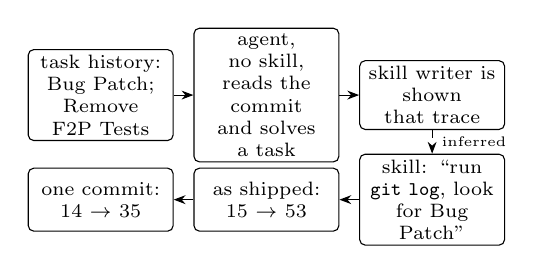
\begin{tikzpicture}[node distance=3mm and 2.5mm, every node/.style={font=\scriptsize,align=center},
  box/.style={draw,rounded corners=2pt,inner sep=2pt,minimum height=8mm,text width=17mm},
  arr/.style={-{Stealth[length=1.5mm]}},inf/.style={arr,dashed}]
\node[box] (env) {task history:\\Bug Patch;\\Remove F2P Tests};
\node[box,right=of env] (agent) {agent, no skill,\\reads the commit\\and solves a task};
\node[box,right=of agent] (refl) {skill writer is\\shown that trace};
\node[box,below=of refl] (skill) {skill: ``run\\\texttt{git log}, look\\for Bug Patch''};
\node[box,left=of skill] (gain) {as shipped:\\\njinjaNone{} $\to$ \njinjaSkill{}};
\node[box,left=of gain] (ctrl) {one commit:\\\njinjaLFNone{} $\to$ \njinjaLFSkill{}};
\draw[arr] (env) -- (agent); \draw[arr] (agent) -- (refl);
\draw[inf] (refl) -- node[right,font=\tiny]{inferred} (skill);
\draw[arr] (skill) -- (gain); \draw[arr] (gain) -- (ctrl);
\end{tikzpicture}
\caption{The mechanism on Jinja. Solid: measured in logs or runs; dashed: inferred, because the
learning call that first wrote the instruction was overwritten. Seed 41, Jinja test split.}
\label{fig:mech}
\end{figure}

\paragraph{What the agent saw}
We audited every saved trace (post hoc; detection rules fixed in the released script and tested on
the false positives of a first version). On the tasks without a description, with the skill in the
shipped environment, the agent displayed the bug-injecting diff in \nhiStudyDiffA{} of
\nhiStudyNA{} runs (seed 41), \nhiStudyDiffB{} of \nhiStudyNA{} (seed 51) and \nhiStudyDiffC{} of
\nhiStudyNC{} (new tasks); it displayed or ran the deleted tests in \nhiStudyTests{} runs. Every
such task it resolved shows the diff in its trace (\nhiStudyResNone{} resolved without it). In
\nhiSingleRuns{} runs in single-commit environments, neither channel appears. Of the resolved
patches on these tasks, \nrvShipNoIssue{} of \nrvShipNoIssueN{} are exact reversals of the bug
patch (\nrvUnseen{} of \nrvUnseenN{} on the new tasks): the agent mostly uses the commit to locate
the bug, not to copy it. These are indicators of use, not proof of it; the interventions below
measure the effect. A cheaper flag, the message ``Bug Patch'' in any observation, agrees with this
audit on \nmonConfAgree{} of \nmonConfN{} saved traces: it is raised on all \nmonConfTP{} runs that
displayed the diff (\nmonConfFN{} missed) and on \nmonConfFP{} runs that saw only the message.

\paragraph{Where it pays off}
On the \njinjaNoPSTasks{} Jinja test tasks without a description, the skill resolves
\njinjaNoPSn{} in the shipped environment and \njinjaNoPSLF{} with one commit; without a skill the
agent resolves \njinjaNoPSNoneBase{} of them (Table~\ref{tab:nops}). The precondition is
common: \nexpoEmpty{} of the \nexpoTasks{} SWE-smith tasks (\nexpoPct\%, in \nexpoRepos{}
repositories) have no description; we measured the effect of the commits on two repositories only.

\begin{table}[t]\centering\footnotesize\setlength{\tabcolsep}{3pt}
\caption{Resolved Jinja tasks without an issue description (scorer $S$). Each row of a block ran in
the same job as the rows it is compared with, except where marked.}\label{tab:nops}
\begin{tabular}{@{}lllr@{}}\toprule
Cohort & Environment & Arm & Resolved\\\midrule
34 test tasks, seed 41 & shipped & no skill & \njinjaNoPSNoneBase{}/\njinjaNoPSTasks\\
 & shipped & learned skill$^{c}$ & \njinjaNoPSn{}/\njinjaNoPSTasks\\
 & shipped & without history line & \nabNoPS{}/\njinjaNoPSTasks\\
 & shipped & relearned skill$^{c}$ & \ncleanShipSolved{}/\ncleanShipN\\
 & one commit & learned skill$^{c}$ & \njinjaNoPSLF{}/\njinjaNoPSTasks\\\midrule
34 test tasks, seed 51 & shipped & learned skill & \nsdNoPS{}/\njinjaNoPSTasks\\
 & three other arms & & \nsdNoPSOther{} each\\\midrule
36 new tasks, seed 51 & shipped & learned / none & \ncfShipSkill{} / \ncfShipNone\\
 & one commit & learned / none & \ncfLFSkill{} / \ncfLFNone\\\bottomrule
\end{tabular}\\[2pt]
\raggedright\footnotesize $^{c}$ran in a different run from the no-skill row of its block.
\end{table}

\subsection{Interventions}\label{sec:interventions}
\paragraph{Removing the two construction commits}
Replacing the history by one commit that holds the buggy tree~\cite{debuggym_swesmith_git_fix}
removes both leak channels and nothing else: there is no project history to remove. On Jinja it
changes the no-skill arm from \njinjaNone{} to \njinjaLFNone{} and the skill arm from \njinjaSkill{}
to \njinjaLFSkill{}; the difference of the two gains, estimated jointly over the same tasks, is
\nleak{} [\nleakLo{}, \nleakHi{}], about \nleakSharePct\% of the gain as shipped. On Bleve the skill
arm falls from \nbleveSkill{} to \nbleveLFSkill{} and the difference is \nbleveLeak{}
[\nbleveLeakLo{}, \nbleveLeakHi{}]; on its \nbleveNoPSN{} tasks without a description the skill
resolves \nbleveNoPS{} with the commits and \nbleveNoPSLF{} without. In J1, J2, B1 and B2 the arms
of a comparison ran in different runs; the same contrast with all four arms in one job is S3
(Section~\ref{sec:replication}).

\paragraph{Separating the message from the diff}
The single-commit control removes the message ``Bug Patch'', its diff and a commit at once. A
registered experiment (C10) rebuilt four histories for the \nctenTasks{} Jinja tasks without a
description, all with the same working tree and the same ``Remove F2P Tests'' commit: A, the shipped
history (rebuilt to the same hashes); B, the same diff under a neutral message from the upstream
history; C, an empty commit named ``Bug Patch'' on the buggy tree, so the pre-bug code is absent; D,
no bug commit. The eight arms (four histories, with and without the skill) ran in one job. The skill
resolves \nctenASkill{} of \nctenASkillN{} tasks in A and \nctenBSkill{}, \nctenCSkill{} and
\nctenDSkill{} in B, C and D; without it, at most \nctenANone{} per history. The registered test
compares A with C, which have the same commits and messages and differ only in whether the pre-bug
code is in the history: over the \nctenACN{} tasks complete in its four arms the difference of gains
favours A on \nctenACNeg{} tasks and C on \nctenACPos{}, mean $D=\nctenACMean{}$ [\nctenACLo{},
\nctenACHi{}], $E=\nctenACE{}\geq 40$: certified. Neither part carries a gain alone: the diff under
a neutral message (B$-$D, $D=\nctenBDMean{}$ [\nctenBDLo{}, \nctenBDHi{}]) and the message without
the diff (C$-$D, $D=\nctenCDMean{}$ [\nctenCDLo{}, \nctenCDHi{}]); the interaction is
\nctenIxMean{} [\nctenIxLo{}, \nctenIxHi{}]. The message leads the agent to the diff: with the skill
it displays the diff in \nctenADiff{} of \nctenASkillN{} runs in A. When no message points to the
diff (B) or no diff exists (C, D), it restores and runs the deleted tests instead in some runs
(\nctenBTests{}, \nctenCTests{} and \nctenDTests{}) and still rarely resolves the task.
Six arms stopped at their spending cap before the last task (our caps left no margin above the
cost estimate), so each contrast uses \nctenACN{} to \nctenBDN{} tasks, as registered. Because the
cut depends on the spend, the end-of-pool guarantee for a fixed pool does not strictly apply; the
same statistic is a test supermartingale under the narrower per-task null, whose guarantee holds
``at all stopping times''~\cite{savi_ramdas_2023}.

\paragraph{Removing the instruction}
A fixed rule deletes every line of the skill that mentions a commit or the history; on the Jinja
skill it deletes exactly one line. With both arms in one job, the skill without it resolves
\nabSkill{} against \nabNone{} (gain \nabGain{}), and \nabNoPS{} of the \njinjaNoPSTasks{} tasks
without a description, against \njinjaNoPSn{} for the full skill. Its gain differs from the full
skill's gain with one commit by \nabVsLF{} [\nabVsLFLo{}, \nabVsLFHi{}]. Deleting a skill line and
deleting history are different interventions, compared here across runs; we read the agreement as
consistent, not as a decomposition.

\paragraph{Removing the leak while learning}
We reran gskill's loop with the settings of the original run and one change: every task container
the loop set up (\ncleanCalls{}, one per metric call) had its history reduced to one commit and
checked (one commit, one reference, no remote, no object carrying the bug-injecting message). None
of the \ncleanCandNonEmpty{} non-empty rewrites kept contains a line about commits or history, and
the skill is certified with one commit (R: \ncleanNone{} to \ncleanSkill{}, $E=\neopG$), though not
at the family threshold. In the shipped environment it resolves \ncleanShipSolved{} of the \ncleanShipN{} tasks
without a description. Each condition had one learning run of a stochastic loop: the absence of the
instruction is an observation on this run, not an estimated rate.

\begin{figure}[t]\centering
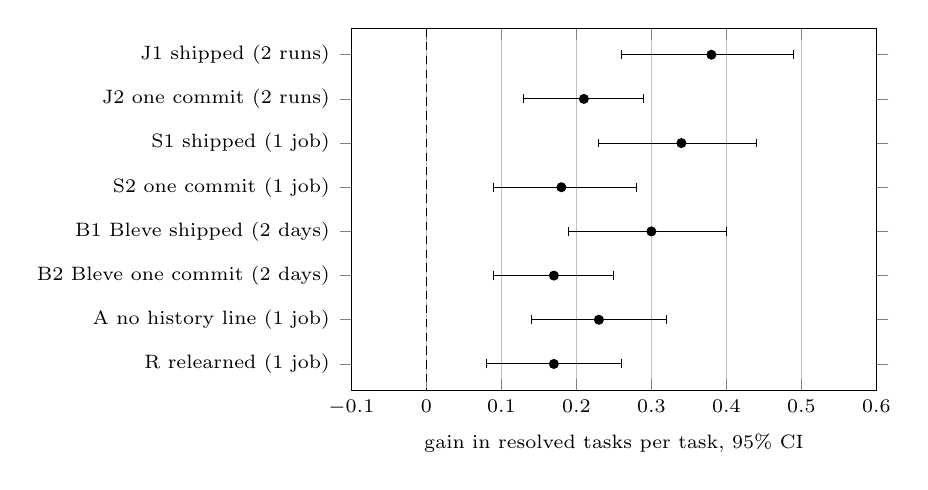
\begin{tikzpicture}
\begin{axis}[width=0.55\linewidth,scale only axis,height=46mm,xmin=-0.1,xmax=0.6,ymin=0.4,ymax=8.6,
  xbar=0pt,y dir=reverse,ytick={1,...,8},
  yticklabels={J1 shipped (2 runs),J2 one commit (2 runs),S1 shipped (1 job),S2 one commit (1 job),
  B1 Bleve shipped (2 days),B2 Bleve one commit (2 days),A no history line (1 job),R relearned (1 job)},
  ticklabel style={font=\scriptsize},xlabel={gain in resolved tasks per task, 95\% CI},
  xlabel style={font=\scriptsize},xmajorgrids]
\addplot[only marks,mark=*,mark size=1.6pt,error bars/.cd,x dir=both,x explicit]
 coordinates {(\njinjaGain,1) -= (\njinjaGain-\njinjaGainLo,0) += (\njinjaGainHi-\njinjaGain,0)
 (\njinjaLFGain,2) -= (\njinjaLFGain-\njinjaLFGainLo,0) += (\njinjaLFGainHi-\njinjaLFGain,0)
 (\nsdGain,3) -= (\nsdGain-\nsdGainLo,0) += (\nsdGainHi-\nsdGain,0)
 (\nsdLFGain,4) -= (\nsdLFGain-\nsdLFGainLo,0) += (\nsdLFGainHi-\nsdLFGain,0)
 (\nbleveGain,5) -= (\nbleveGain-\nbleveGainLo,0) += (\nbleveGainHi-\nbleveGain,0)
 (\nbleveLFGain,6) -= (\nbleveLFGain-\nbleveLFGainLo,0) += (\nbleveLFGainHi-\nbleveLFGain,0)
 (\nabGain,7) -= (\nabGain-\nabGainLo,0) += (\nabGainHi-\nabGain,0)
 (\ncleanGain,8) -= (\ncleanGain-\ncleanGainLo,0) += (\ncleanGainHi-\ncleanGain,0)};
\draw[densely dashed] (axis cs:0,0.4) -- (axis cs:0,8.6);
\end{axis}
\end{tikzpicture}
\caption{Paired gains with 95\% task-level bootstrap intervals, 100 tasks each (scorer $S$). Pairs of
rows differ only in the history (J1/J2, S1/S2, B1/B2). Arms in one job (S1, S2, A, R) or in
different runs (J, B).}
\label{fig:effects}
\end{figure}

\subsection{Replication and a confirmatory test}\label{sec:replication}
With a second agent seed, all four Jinja arms in one job, the skill is confirmed in both
environments (S1, S2; Holm at 0.025) and the difference of the gains is \nsdLeak{} [\nsdLeakLo{},
\nsdLeakHi{}], against \nleak{} on the first seed. The registered contrast over all 100 tasks (S3)
is not significant ($E=\neopK$; anytime-valid $p=\nsdEnvP$): at $n=100$ and a difference of this size
it has little power.

Before opening any result of the second seed we registered one confirmatory test where the
mechanism predicts the contrast: the \ncfOld{} test tasks without a description, \emph{already used}
with seed 41 and now run with seed 51, followed by \ncfNew{} Jinja tasks never used in this study
(the first \ncfNew{} tasks without a description after the rows gskill samples, in dataset order),
in the same four arms (Figure~\ref{fig:timeline}). The pool is the concatenation of two fixed
cohorts in a fixed order, not a random permutation, so we read the registered e-process for the
null that no task favours the environment as shipped, and the end-of-pool test for the null on the
pool mean. \ncfFor{} tasks favour the environment as shipped and \ncfAgainst{} the single commit
($E=\neopL$; the e-process crossed 40 at task \ncfCross{}, $p=\ncfP$). By cohort: \ncfOldFor{} of
the \ncfOld{} known tasks and \ncfNewFor{} of the \ncfNew{} new tasks favour the shipped environment,
none the other (exact sign test on the new cohort, $p=\ncfNewSignP$, post hoc). On the new tasks the
skill resolves \ncfShipSkill{} as shipped and \ncfLFSkill{} with one commit, against \ncfShipNone{}
and \ncfLFNone{} without it.

\begin{figure}[t]\centering
\resizebox{\linewidth}{!}{%
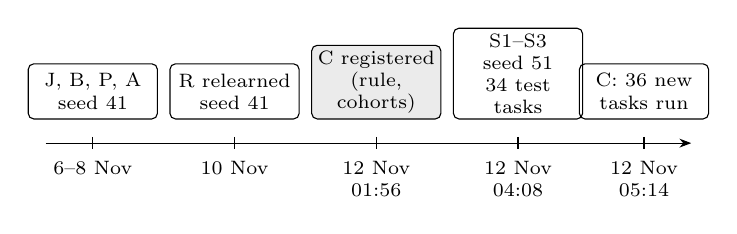
\begin{tikzpicture}[every node/.style={font=\scriptsize,align=center},
  ev/.style={draw,rounded corners=2pt,inner sep=2pt,text width=15mm,minimum height=7mm}]
\draw[-{Stealth[length=1.5mm]}] (0,0) -- (8.2,0);
\foreach \x/\l in {0.6/{6--8 Nov},2.4/{10 Nov},4.2/{12 Nov\\01:56},6.0/{12 Nov\\04:08},7.6/{12 Nov\\05:14}}
  {\draw (\x,0.08) -- (\x,-0.08); \node[below] at (\x,-0.1) {\l};}
\node[ev,above] at (0.6,0.3) {J, B, P, A\\seed 41};
\node[ev,above] at (2.4,0.3) {R relearned\\seed 41};
\node[ev,above,fill=black!8] at (4.2,0.3) {C registered\\(rule, cohorts)};
\node[ev,above] at (6.0,0.3) {S1--S3 seed 51\\34 test tasks};
\node[ev,above] at (7.6,0.3) {C: 36 new\\tasks run};
\end{tikzpicture}}
\caption{Chronology of the Jinja experiments. The confirmatory test C was committed before any
result of the second seed was opened; its pool is the 34 test tasks without a description (seed 51)
followed by 36 new tasks. Times are UTC commit and publication times.}
\label{fig:timeline}
\end{figure}

\subsection{What persists under the control}\label{sec:residual}
Without the two commits, the Jinja skill still raises the resolved count from \njinjaLFNone{} to
\njinjaLFSkill{} and is certified (J2), as are the Bleve skill (B2) and the second-seed replicate
(S2). This part of the gain persists under the single-commit control according to $S$. It is not
explained by the length of the prompt as far as one control can show: replacing the skill by the
only public SWE-Skills-Bench skill within $\pm5\%$ of its length~\cite{webdev_skills_bench_2026}, a
Go concurrency guide that says nothing about Jinja, the agent resolves \nplcS{} tasks; the learned
skill's content effect is \nconGain{} [\nconGainLo{}, \nconGainHi{}], and this particular irrelevant
skill's effect is \nlenGain{} [\nlenGainLo{}, \nlenGainHi{}] ($p=\nlenP$, two-sided). One placebo
does not estimate the variation of irrelevant prompts, and the placebo arm ran a day after the arms
it is compared with.

\subsection{Scope}\label{sec:scope}
\paragraph{Another repository}
Reused verbatim on the \npygN{} Pygments test tasks, the Jinja skill resolves \npygSkill{} against
\npygNone{} (registered two-sided test, $p=\npygP$; gain \npygGain{} [\npygGainLo{}, \npygGainHi{}])
and is not certified; gskill's scorer $L$ reports \npygLSkill{} against \npygLNone{}. With a base
rate of \npygNone{} in 100 this test has little power to detect harm: it shows an absence of
evidence for transfer to this repository under this scorer, not equivalence, and says nothing about
other repositories.

\paragraph{Another agent model}
\flashmodel{}, on the \nflN{} tasks without a description (registered, descriptive), resolves
\nflSkill{} with the skill and \nflNone{} without, against \njinjaNoPSNoneBase{} for our agent. It
uses both channels without any skill: it displayed the bug-injecting diff in \nhiFlNoneDiff{} of
\nflN{} no-skill runs and the deleted tests in \nhiFlNoneTests{}, and ran a command that restores
files from the history in \nhiFlNoneRestore{} (\nhiFlSkillTests{} runs with the deleted tests
displayed with the skill). We did not run the single-commit control for this model, so how much of
its \nflNone{} resolved tasks the commits explain is not measured.

\paragraph{Other agent--model configurations (post hoc)}
SWE-Skills-Bench publishes one run per skill for \nsskbConfigs{} configurations~\cite{sskb_paper}.
On its \nsskbSkills{} common skills only about \nsskbRhoPct\% of the variance of skill effects is
shared between configurations ($\rho=\nsskbRho$); where a skill changes the pass rate by at least
\nsskbThr{} points in one configuration, another shows a change of that size in the same direction
in \nsskbSamePct\% of cases and in the opposite direction in \nsskbOppPct\%. With one run per
configuration these figures cannot separate scope from noise.

\paragraph{The instruction travels without the gain}
On Pygments, the Jinja skill led the agent to the ``Bug Patch'' commit in \nmonPygFlag{} of
\nmonPygRuns{} runs (\nmonPygNoneFlag{} without the skill), and \nmonPygSolved{} of these runs were
resolved. In the single-commit Bleve environment the skill still sent the agent to the history
(\texttt{git log} or \texttt{git show} in \nmonCmdBleve{} of \nmonCmdBleveRuns{} runs), with nothing
to find.

\subsection{Measurement controls}\label{sec:measurement}
\paragraph{The scorer of a learning pipeline}
gskill's public scorer at commit 8c7b697 marks a patch as passing whenever the test output contains
``passed'' in any letter case, unless it also contains ``Patch Apply Failed''~\cite{gskill_swe_harness}.
A no-op patch passes on \nfzeroLNoop{} of \nfzeroN{} tasks across \nfzeroRepos{} SWE-smith
repositories; $S$ passes \nfzeroSNoop{} of them and passes the gold patch on at least
\nfzeroGoldMinPct\% of the tasks of every repository. On the agent's patches, $L$ reports
\njinjaLNone{} and \njinjaLSkill{} on Jinja where $S$ finds \njinjaNone{} and \njinjaSkill{}. We make
no claim about the numbers in the pipeline's announcement.

\paragraph{Decision rules: what each is for}
Table~\ref{tab:rules} compares the rules by error control, each at its own intended level and number
of looks; these are not comparisons of learning algorithms.

\begin{table}[t]\centering\footnotesize\setlength{\tabcolsep}{2.5pt}
\caption{Decision rules. A/A: false admissions on \naaStreams{} resampled A/A streams of
\naaTrials{} trials. Orders: largest share of \npermN{} random orders of the \nrulesNull{} collected
A/A streams that a rule admits (post hoc).}\label{tab:rules}
\begin{tabular}{@{}llllrr@{}}\toprule
Rule & Intended use & Level & Looks & A/A & Orders\\\midrule
Plug-in, mean favours skill & quick check & none & 1 & \npluginOnce & --\\
Plug-in, monitored & & none & every \naaLook & \npluginMonitored & --\\
Mantel--Haenszel gate$^{d}$ & interval & 2.5\% & 1 & \nbxOnce & --\\
Mantel--Haenszel, monitored & & 2.5\% & every 10 & \nbxMonitored & \nrulesMHAAMax\%\\
GEPA acceptance & search & none & 1 (3 tasks) & \ngepaNoop$^{e}$ & \nrulesGepaAAMax\%\\
Exact sign test, monitored & fixed-$n$ test & 2.5\% & every 10 & -- & \nrulesSignAAMax\%\\
Gatekeeper e-process & sequential & 2.5\% & every task & \ngkAdmitAA & \nrulesGkAAMax\%\\
End-of-pool test & fixed pool & 2.5\% & 1 (end) & -- & --\\\bottomrule
\end{tabular}\\[2pt]
\raggedright\footnotesize $^{d}$built by us from XRepoSkill's statistic, which XRepoSkill does not
use as a threshold. $^{e}$share of proposals that change nothing that are accepted.
\end{table}

\paragraph{Decision rules under A/A}
From \naaTasks{} tasks with three no-skill runs each we built \naaStreams{} A/A streams of
\naaTrials{} paired trials. These are comparisons of error control, not of learning algorithms:
each rule is read at its intended level. A plug-in rule that admits when the mean difference
favours the skill admits in \npluginOnce{} of the streams after \naaTrials{} trials, and in
\npluginMonitored{} when looked at every \naaLook{} trials; a Mantel--Haenszel gate built from
XRepoSkill's statistic (lower end of a two-sided 95\% interval above 0) admits in \nbxOnce{} at one
look and \nbxMonitored{} when monitored; GEPA's acceptance rule, inside the learning loop and not
designed for error control, accepts \ngepaNoop{} of proposals that change nothing (under A/A a
proposal that changes nothing is accepted with probability $(1-\Pr[\text{tie}])/2$, which grows
towards $1/2$ with the minibatch); the registered e-process admits in \ngkAdmitAA{}. On the
\nrulesStreams{} streams collected for this paper (post hoc; labels fixed before the replay:
\nrulesPos{} confirmed effects, \nrulesNull{} A/A, \nrulesHarm{} harmful by design), the
e-process, the sign test and the Mantel--Haenszel gate decide alike in the order run; the plug-in
rule admits \nrulesPluginNull{} of the A/A streams and GEPA's rule \nrulesGepaPos{} of the
\nrulesPos{} positive ones. On effects of this size the e-process reaches the same decisions as a
fixed-sample test; what it adds is the right to stop, which, all tasks having been run, we can only
assess retrospectively (first crossings after \nadmitMeanTrials{} tasks on average).

\paragraph{Our own harness}
No-op patches resolve \nnoopOurs{} of \nnoopOursN{} tasks and gold patches \ngoldOursOk{} of
\ngoldOursN{}. Rescoring all \nrsPatches{} non-empty Jinja patches twice changed \nrsFlips{} of
\nrsScorings{} outcomes.

\paragraph{Attribution and rerun noise}
A published procedure flags a failure as skill-induced when the run with the skill fails a task that
a reference run solves~\cite{skill_induced_failures_2026}. Applied to two runs \emph{without} any
skill, it flags \nattrPlacebo{} candidates against \nattrSkill{} with a skill on \nattrTasks{}
SWE-bench-Live tasks (ratio \nattrR{}, 95\% interval [\nattrRLo{}, \nattrRHi{}]). LLM auditors shown a
sham skill that by construction caused nothing blamed it for \nshamLiteK{} of \nshamLiteN{},
\nshamFlashK{} of \nshamFlashN{} and \nshamProK{} of \nshamProN{} failures (\agentmodel{},
\flashmodel{}, \promodel{}). For a benchmark of $n$ tasks, the rerun noise is the 97.5th percentile
of the absolute difference in resolve rate between two no-skill runs, resampled from our runs on
\nnoiseTasks{} tasks: \nnoiseWithin{} of \nnoiseClaims{} gains reported for XRepoSkill and
MemGovern~\cite{xreposkill,memgovern_repo} are no larger than this level at their $n$. This is an
indication measured with our agent, not a test of those papers. For MemGovern, a registered
manipulation check (the agent must call the memory tools) failed on our harness (\nmgUsed{} of
\nmgRuns{} runs), so we did not evaluate it; this says nothing about MemGovern with its own harness.

\section{Discussion}
\paragraph{A statistical gate certifies a gain, not its source}
A gate such as PACE~\cite{pace_paired_anytime_gate} or Gatekeeper answers whether a change raises
the score on the evaluation tasks. It cannot answer whether the rise comes from a capability or from
information the evaluation environment should not provide: in the learning environment the
leak-seeking instruction does raise the resolved count, so a valid gate inside the loop would accept
it, at a higher cost (the registered e-process needed \njinjaAdmit{} to \nbleveLFAdmit{} paired
tasks where GEPA uses three, retrospectively). Only a control in which the claimed cause is absent
separates the two. Applied to the learning environment, the single-commit control removed the
instruction before it was written.

\paragraph{The cost of re-certification}
A change of scope means a new certification. With our agent a paired task cost on average
\ntokTrialIn{} thousand input and \ntokTrialOut{} thousand output tokens; the registered e-process
would have stopped after \nadmitMinTrials{} to \nadmitMaxTrials{} paired tasks, that is
\ntokAdmitLo{} to \ntokAdmitHi{} million input tokens per scope. These are retrospective: every
comparison ran all its tasks.

\paragraph{What a certification is worth}
A certification here is a statement about a fixed pool of tasks within one run (T1). It is not a
statement about future runs: the model behind the same name changed between our earlier and later
runs (a registered check found identical first responses on \ndriftMatch{} of \ndriftTasks{} tasks),
and the replication with a second seed is descriptive evidence of stability, not a guarantee. It is
not a statement about other tasks or repositories: the Pygments reuse and the second agent show how
far a scope can differ.

\section{Threats to Validity}\label{sec:threats}
\paragraph{Measurement}
Gains are under the benchmark's tests ($S$), which we checked with no-op and gold patches but not
with an independent semantic check. Tasks are synthetic, from three repositories; base rates without
a skill are low (\njinjaNone{}, \nbleveNone{}, \npygNone{} of 100), so the tests have little power to
detect harm. We could not verify the model's training cutoff and make no claim that tasks are unseen.

\paragraph{Interventions}
The single-commit control removes both construction commits at once. C10 separates the message of
the bug-injecting commit from its diff on one repository, one skill and one seed; it keeps the
``Remove F2P Tests'' commit in every history, so that channel was not varied.
Other channels (image artefacts, file names, timestamps) were not probed. One learning run per
condition: the presence or absence of the instruction is an observation, and the learning calls of
the first half were overwritten. The reflection model was not varied.

\paragraph{Inference}
The certification rests on Assumption~\ref{ass:indep} given the run state, which diagnostics can
challenge but not establish; runs of different tasks share a provider and its rate limits. The
end-of-pool test is a post hoc reanalysis of registered comparisons. Comparisons whose arms ran in
different runs (J, B, P) include the difference between runs in T1; S1--S3, A and R do not. Holm's
procedure over the registered sign tests does not control the error of the e-process decisions;
Table~\ref{tab:decisions} reports both readings.

\paragraph{Scope}
One agent model for the confirmatory runs; the descriptive runs with \promodel{} and \flashmodel{}
are of the same vendor. Whether other vendors' models learn or follow the instruction is open.

\section{Related Work}
Skill libraries go back to Voyager~\cite{voyager}; for coding agents, skills are mined from
trajectories~\cite{xreposkill}, stored as cards~\cite{memgovern_repo} or optimised against a
benchmark~\cite{gskill}. SWE-Skills-Bench measures skills by one run per configuration~\cite{sskb_paper},
SkillsBench across tasks~\cite{skillsbench_2026}, and SkillJuror how a skill's organisation changes
behaviour~\cite{skilljuror_2026}. Closest to gskill, Kozyrev et al.\ optimise repository skill files
with GEPA, run every attempt ``on an isolated checkout at the frozen base with .git removed'', and
report that one score ``wrote the training pull requests back into prose''~\cite{skill_issue_2026};
our single-commit control is close to that setup, and we measure how much of a certified gain the
history accounts for. Run-to-run variance~\cite{randomness_agentic_evals_2026}, the
harness~\cite{same_model_harness_2026} and tests that accept incorrect
patches~\cite{patchdiff_2025,utboost_2025,test_overfitting_2025} move resolve rates. Git-history
leaks are documented for SWE-bench~\cite{swebench_git_log_leak,swebench_git_log_fix}, SWE-Bench
Pro~\cite{swebench_pro_verified}, other benchmarks~\cite{cursor_reward_hacking,
poolside_benchmark_hacking} and SWE-smith~\cite{marin_swesmith_git_leak,debuggym_swesmith_git_leak,
debuggym_swesmith_git_fix,rllm_hide_git_history}; these works study agents that find a leak, and
hack-verifiable environments plant such opportunities by design~\cite{hack_verifiable_2026}. Paired
anytime-valid gates accept changes of self-evolving agents (PACE~\cite{pace_paired_anytime_gate})
and investment factors~\cite{anytime_referee_2026}; e-processes certify the performance of one
system~\cite{celeus_2026,evaluator_2025}. HDSO and Library Drift accept or retire skills by
validation and outcome floors~\cite{hdso_2026,library_drift_2026}. We add controls in which the
claimed cause of a gain is absent, and state what such a certification covers.

\section{Conclusion}
A resolve-rate gain certifies a skill only in the scope where it was measured, and the evaluation
environment is part of that scope. On SWE-smith a published learner turned two construction commits
into advice: on Jinja, \nleak{} of a \njinjaGain{} gain depends on them, a second seed and a
preregistered test on tasks without a description confirm the difference, and a Go skill repeats
the pattern. The rest of each gain persists without the commits and is certified for its pool and
run. A stronger agent reads both commits with no skill. Evaluating a learned skill therefore needs
controls in which the claimed cause is absent, and a statement of what the certification covers.

\section*{Data Availability}
An anonymized replication package accompanies the submission: the preregistrations with the commit
time of every registration, the analysis scripts, the raw runs and traces, and the scripts that
generate every number in this paper. Third-party texts without a licence are not redistributed.

\section*{Use of AI Tools}
AI coding assistants were used to write the experiment and analysis code, to run the analyses and to
draft text. Every number in the paper is generated by a script from the raw results; the
preregistrations, the code and the generated numbers were reviewed by the author.

\bibliographystyle{ACM-Reference-Format}
\bibliography{refs}
\end{document}
